\documentclass{report}

%%%%%%%%%%%%%%%%%%%%%%%%%%%%%%%%%%%%
% Accents français
%%%%%%%%%%%%%%%%%%%%%%%%%%%%%%%%%%%%
\usepackage[utf8]{inputenc}
\usepackage[T1]{fontenc}
\usepackage{graphicx}

%%%%%%%%%%%%%%%%%%%%%%%%%%%%%%%%%%%%
% Todo notes
%%%%%%%%%%%%%%%%%%%%%%%%%%%%%%%%%%%%
% \usepackage[textwidth=17mm]{todonotes}
% \newcommand{\customtodo}[4]{
%         \todo[color=#2,inline,size=\small]{
%                 \ifx&#3&
%                         \textbf{#1} #4
%                 \else
%                         \textbf{#1$\Rightarrow$#3} #4
%                 \fi
%         }
% }
\newcommand{\AL}[2][]{\customtodo{AL}{green!50}{#1}{#2}}
\newcommand{\JP}[2][]{\customtodo{JP}{red!20}{#1}{#2}}
\newcommand{\FD}[2][]{\customtodo{JP}{brown!20}{#1}{#2}}
\newcommand{\LP}[2][]{\customtodo{MB}{orange!20}{#1}{#2}}

\newcommand{\ie}[0]{{\em i.e.},\xspace}
\newcommand{\vs}[0]{{\em vs.}\xspace}
\newcommand{\eg}[0]{{\em e.g.},\xspace}
\newcommand{\etal}[0]{{\em et al.}\xspace}
\newcommand{\wrt}[0]{{\em w.r.t.}\xspace}
\newcommand{\aka}[0]{{\em a.k.a.}\xspace}

\usepackage{bera}% optional: just to have a nice mono-spaced font
\usepackage{listings}
\usepackage{xcolor}

\colorlet{punct}{red!60!black}
\definecolor{background}{HTML}{EEEEEE}
\definecolor{delim}{RGB}{20,105,176}
\colorlet{numb}{magenta!60!black}

\lstdefinelanguage{json}{
    basicstyle=\normalfont\ttfamily,
    numbers=left,
    numberstyle=\scriptsize,
    stepnumber=1,
    numbersep=8pt,
    showstringspaces=false,
    breaklines=true,
    frame=lines,
    backgroundcolor=\color{background},
    literate=
     *{0}{{{\color{numb}0}}}{1}
      {1}{{{\color{numb}1}}}{1}
      {2}{{{\color{numb}2}}}{1}
      {3}{{{\color{numb}3}}}{1}
      {4}{{{\color{numb}4}}}{1}
      {5}{{{\color{numb}5}}}{1}
      {6}{{{\color{numb}6}}}{1}
      {7}{{{\color{numb}7}}}{1}
      {8}{{{\color{numb}8}}}{1}
      {9}{{{\color{numb}9}}}{1}
      {:}{{{\color{punct}{:}}}}{1}
      {,}{{{\color{punct}{,}}}}{1}
      {\{}{{{\color{delim}{\{}}}}{1}
      {\}}{{{\color{delim}{\}}}}}{1}
      {[}{{{\color{delim}{[}}}}{1}
      {]}{{{\color{delim}{]}}}}{1},
}


\sloppy

\usepackage{xspace}
\usepackage{url}
\usepackage{paralist}
\usepackage{rotating}
\usepackage{tikz}

\begin{document}

% \title{Integrating NoSQL databases in OpenStack Nova}

% % \numberofauthors{4}
% \author{
% %
% % 1st. author
% % \alignauthor
% Jonathan Pastor\\
%        \affaddr{ASCOLA Research Group}\\
%        \affaddr{Mines Nantes / Inria / LINA UMR 6241}\\
%        \affaddr{Nantes, France}\\
% }

\title{Integrating NoSQL databases in OpenStack Nova}
\author{Jonathan Pastor}


\maketitle

\tableofcontents

\begin{abstract}

The objective of this document is to provide a technical description of how we
integrated a NoSQL solution in OpenStack. It will first introduce how OpenStack
works, how several controllers can work together, and finally what was the 
strategy choosed to replace the relational backend with a NoSQL backend.
% \keywords{Cloud computing, IaaS Architecture, OpenStack, NoSQL, Peer
%   to Peer}
\end{abstract}


%% Comment this line for submission
%\listoftodos

\chapter{Introduction}
\label{sec:intro}

OpenStack is an opensource project that aims at developing a complete cloud
management system. Similary to the reference architecture described in the
previous Section, it is composed of several services, each one dealing with a
particular aspect a CC infrastructure as depicted in Figure~\ref{fig:openstack}.

\begin{figure}[htbp]
        \centering
        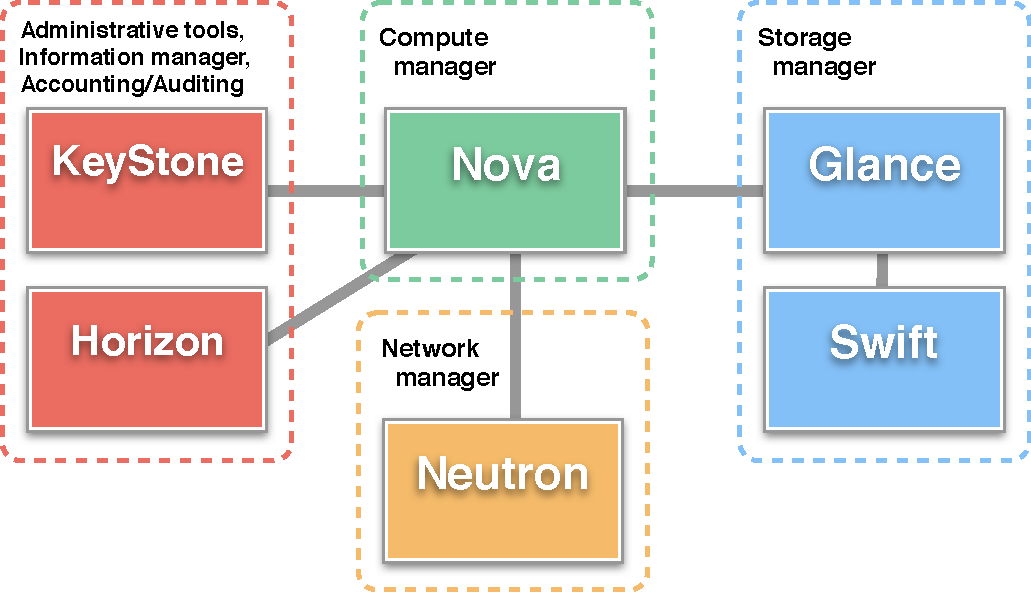
\includegraphics[width=10cm]{figures/OpenStack_architecture.pdf}
        \caption{Services composing OpenStack.}
        \label{fig:openstack}
\vspace*{-.3cm}
\end{figure}


OpenStack relies on two kinds of nodes: controller and compute node. The former
is in charge of managing and distributing work to the latter that provides
computing/storage resources to end-users. In other words, the controllers
correspond to the different services introduced in the previous section while
the compute nodes host the VMs. From the software point of view, the OpenStack
architecture is based on the ``shared nothing" principles: each controller (\ie
each service) is connected to the others via two different way:

\begin{itemize}
   \setlength{\itemsep}{0pt}
  \setlength{\parskip}{0pt}
   \setlength{\parsep}{0pt}
\item \textbf{A messaging queue} that enables the collaboration between sub-services of a
  controller.
\item \textbf{A SQL database} (DB) that stores inner states of a controller.
\end{itemize}

OpenStack's controllers interact with each other through REST APIs or directly
by accessing the inner-state that are stored in the differents DBs. The
architecture used for the Nova service has been organised in a way which ensures
that each of its sub-services does not directly manipulate the database: they
have an indirect access through a service called ``nova-conductor" which in turn
works with an implementation of the \textbf{"nova.db.api"} programming
interface. Developers of Nova provide an implementation of this interface that
is using \textit{SQLAlchemy} to manipulate a relational database. We developed a
second implementation of this interface that replaces every call to the
\textit{SQLAlchemy} by a call to a custom RIAK driver. This enables to make
Nova's services working with RIAK by only changing the database driver: this
limits the level of intrusiveness in the original source code.


\chapter{Collaboration between Nova controllers}
\label{sec:collaboration}



\section{Organisation of the collaboration between components of OpenStack}

Collaboration between components of OpenStack is based on three different ways:
AMQP \footnote{AMQP: Advanced Messaging Queuing Protocol} bus, HTTP APIs and
sharing of inner-states via a replicated relational databases. Each of the 
preceding way of collaborating have specific purposes: some are intended for 
local collaboration as with sub-services of a controller, while some of these
ways are intended for inter-controller collaboration.

\subsection{AMQP bus: making sub-services collaborating}

\subsection{HTTP APIs: making sub-services collaborating}

\subsection{Shared inner-states: collaboration between remote controllers}


\section{Creation of a VM: detailed workflow}

During the study of OpenStack components, it was noticable that a large part of
the collaboration that happend between controllers during the creation of a VM
\footnote{VM: Virtual machine} was done via the sharing of inner-states.

\begin{sidewaysfigure}[htbp]
        \centering
        %http://www.websequencediagrams.com/?lz=dGl0bGUgQ3JlYXRpb24gb2YgYSBWTQoKVXNlciAtPiArY29uZHVjdG9yLm1hbmFnZXIqXG5AZWNvbm9tZTE1OiBidWlsZF9pbnN0YW5jZSgpCgATHgBPBXNjaGVkdWxlci5maWx0ZXJfAAgJAE4PACAJX3J1bgBZDAAbJwCBOwdtcHV0ZQCBLRM3OiAASQ8KIyBCdWlsZCAAgUkICgAjGy0-AD4eXwCCCxEKICAAKiZyZXNzb3VyY2VfdHJhY2tlcgCBKA0AgmYIX2NsYWltKCkATAsAHRwtPi0AgW8dAEYIAH0pAIFgFmFsbG9jYXRlX25ldHdvcmsAgRsFAIFZIAAlBwCDDxYASQlmb3IAhF8MICAgIAAeGy0-ADAmbWFjX2FkZHJlc3MAC0pmaXhlZF9pcABmQXVwZGF0ZV9kbgB4JQCDRB4AgwsHX2luZm8AhGwgAIQPHQCFKSEAhEweX3ByZXBfYmxvY2tfZGV2aQCDRwcAhjA8c3Bhd24AhEYldmlydC5kcml2AIZHDwA2DAAOFi0AhiIgb2s&s=default
        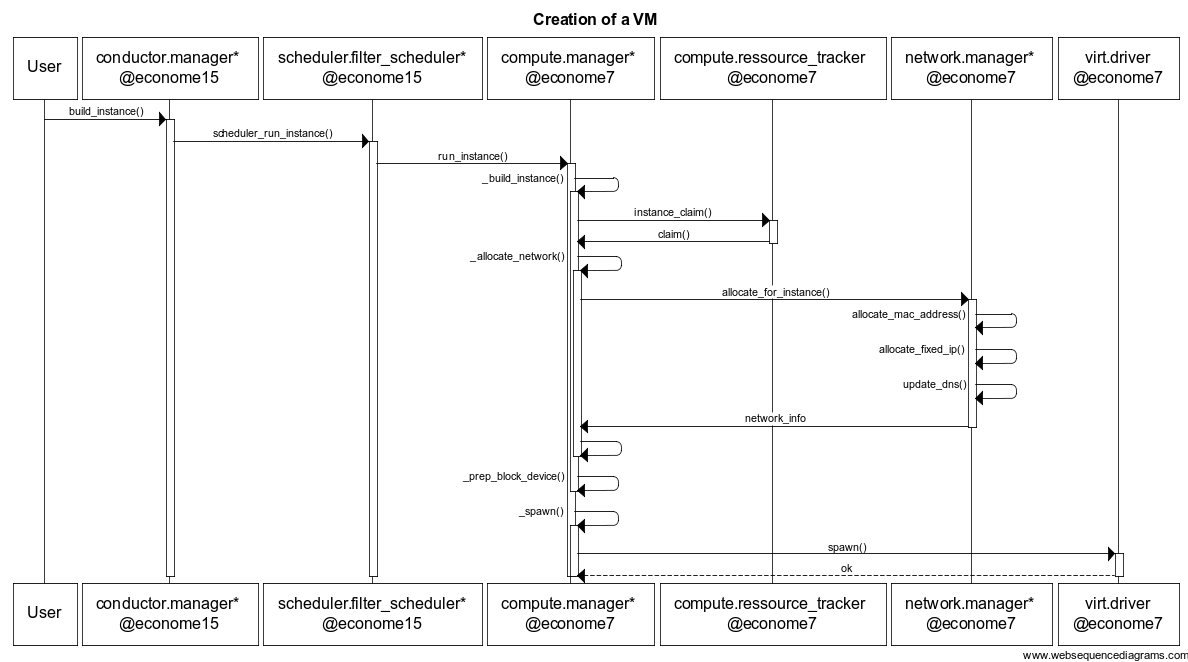
\includegraphics[width=23cm]{figures/sequence.png}        
        \caption{Services involved in the creation of a VM.}
        \label{fig:sequence_vm_creation}
\vspace*{-.3cm}
\end{sidewaysfigure}

Indeed, when a request for the creation of a VM was made, the \emph{nova-api}
sub-service performed actions that resulted in the storage of an VM object in
the database. A simplified view of this VM object can be found in the following
listing:

\begin{lstlisting}[language=json,firstnumber=1]
{
   'hostname':u'vm1',
   'vm_state':u'building',
   'progress':0,
   'project_id':u'1b46e91b72984e47ad0d8d127f59e978',
   'launched_at':None,
   'scheduled_at':None,
   'deleted':0,
   'key_name':None,
   'task_state':u'scheduling',
}
\end{lstlisting}

It is noticable that this object as

\chapter{Propostion: leveraging ROME to replace the relational backend}
\label{sec:leveraging-rome}

The current implementation of Nova is based on a relational database. To enable
Nova to work with several controllers, this database is replicated on each
server hosting a Nova controller, thanks to the Galera project
\footnote{http://galeracluster.com/} The architecture used for the Nova service
has been organised in a way which ensures that each of its sub-services does not
directly manipulate the database: they have an indirect access through a service
called ``nova-conductor" which in turn works with an implementation of the
\textbf{"nova.db.api"} programming interface. Developers of Nova provide an
implementation of this interface that is using \textit{SQLAlchemy} to manipulate
a relational database.

Leveraging the software interfaces provided by \textit{SQLAlchemy}, we developed
the ROME project: it target at delivering a small driver for key/value stores.
We aim at integrating OpenStack Nova with NoSQL backend without modifying
OpenStack's core code. We build a prototype of this driver and made Nova use it
during validations on the Grid'5000 testbed: to develop this prototype we
changed code only in the \textbf{"nova.db.api"} class, to add call to the ROME
driver.

\begin{figure}[h!]
        \centering
        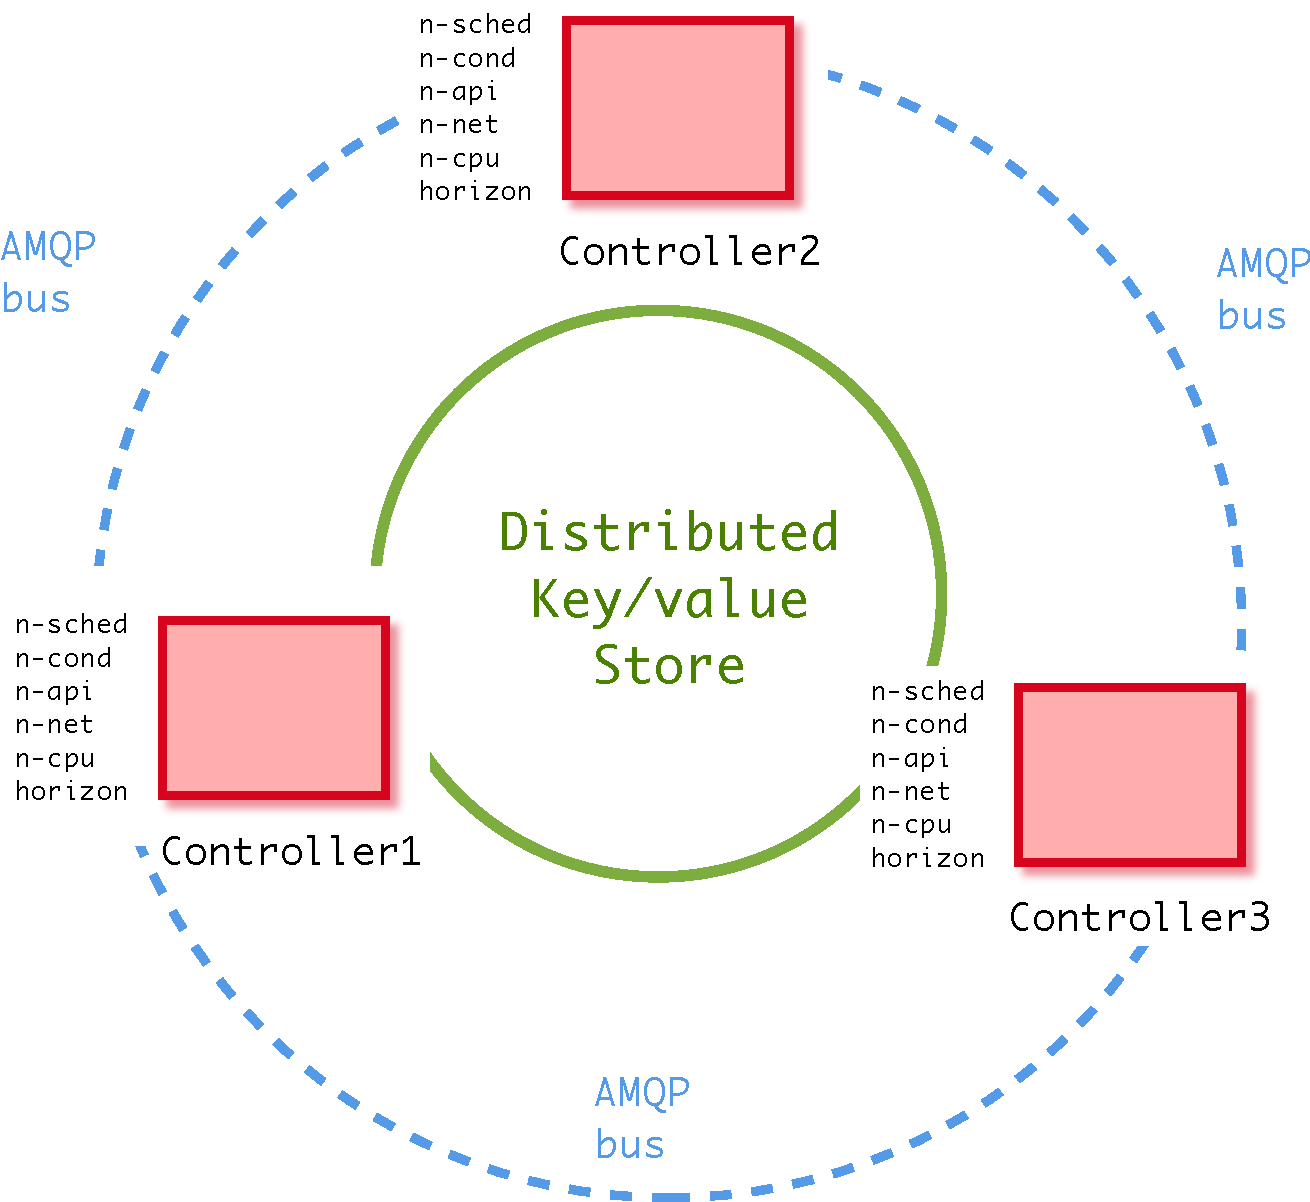
\includegraphics[width=10cm]{figures/OpenStack_distributed.pdf}
        \caption{Nova controllers are connected through a shared key/value backend
        and the AMQP bus.}
      \label{fig:newnova}
\vspace*{-.3cm}
\end{figure}

\section{Mechanisms behind ROME}

\subsection{How the storage works?}

In order to ensure a compatibility between objects manipulated by the relational
driver and our driver, models leverage the same base class as in the relational
driver. Thus all objects that are supposed to be stored in a non relational
database must extends the \emph{oslo.db.sqlalchemy.models.ModelBase} class which
provides:

\begin{itemize}
\item save function.
\item update function.
\item \emph{"dictionnary like"} behaviour.
\end{itemize}

When an entity object is saved, the ROME driver will marshall it in JSON format:
each of its fields will be translated in JSON value. This transformation is
trivial with integer, string, boolean and lists, but become more complex with
relationships. When the rome driver encounter an object A linked with a remote
object B via a relationship, it will transform the relationship to B with a
\emph{link} object that contains enough information to retrieve the remote
object and then check if b has been modified in order to save its changes. This
mechanisms is illustrated in figure \ref{fig:rome_marshalling}

\begin{figure}[h!]
        \centering
        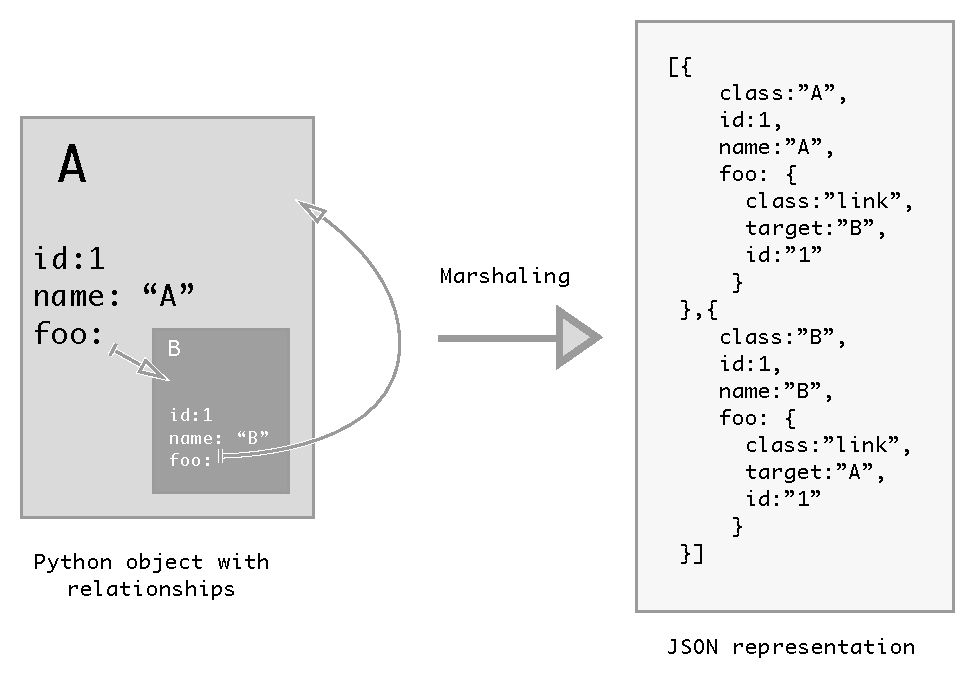
\includegraphics[width=10cm]{figures/rome_marshaling.pdf}
        \caption{An object containing relationships to another object is
        converted to the JSON format and then saved in database.}
      \label{fig:rome_marshalling}
\vspace*{-.3cm}
\end{figure}

Once the object has been marshalled, it can be saved in any Key/value store
(KVS): if the KVS support JSON storing, then no transformation is needed,
otherwise it is possible to store the JSON as a string. Keeping a JSON format is
important as it is a widely supported format, which is good for 
interoperability.

This JSON data is store in the bucket that corresponds to its original class:
every objects of the same class will be stored in the same bucket.

\subsection{How objects are queried?}




\chapter{Future work}
\label{sec:future_work}

\subsection{Improve reactivity of the ROME driver}


\subsection{Toward a "smooth" integration of the driver in OpenStack}



\chapter{Conclusion}
\label{sec:conclusion}

This document gives an unformal view of what have been done for making OpenStack
leverage NoSQL databases. This document focus exclusively on the Nova service.
Our work has led us to first study how services in OpenStack collaborate and 
then to develop \emph{ROME}, an extension for KVS that enables
them to be used with the same interfaces as provided by emph{SQLAlchemy}. The
mechanisms that are used in ROME are described, and improvements are proposed in
section \ref{sec:future_work}.

\bibliographystyle{abbrv}
\bibliography{main}

\end{document}
